%*******************************************************************************
%*********************************** Fifth Chapter *****************************
%*******************************************************************************

\chapter{Results and Discussions}  %Title of the Fifth Chapter

\section{Results}
    These are the different results of the experiments on the model. The indications of these results will then be discussed and analyzed.

    The first set experiments will focus on the different cell dimensions as the experimental variable. The period and seasonality of data will be controlled variables. The timestep will be set to monthly and the seasonality to false.

    \begin{table}[H]
      \centering
      \begin{tabular}{|c|c|c|c|}
            \hline
          \textbf{Cell Dimension}  &\textbf{MSE}  &\textbf{Accuracy} &\textbf{F1 Score}\\ 
          \hline
          500x500m &1.13 &88.98 &89.15 \\
          750mx750m &0.87 &91.78 &92.3 \\
          1000mx1000m  &0.98 &89.01 &90.36 \\
          \hline
        \end{tabular}
      \caption{Performance of the model for different cell dimensions}
    \end{table}
    Table 4.1 shows the results of the experiments for the different cell dimensions. The difference cell dimensions are 500mx500m, 750mx750m, 1000mx1000m. The model performs highest with 750mx750m cell dimension with an accuracy of 91.78 and F1 score of 92.3.

    The next set experiments will focus on the different timesteps. The cell dimension and seasonality will now be controlled variables. The cell dimension will be set to 1000mx1000m and the seasonality to false.

    \begin{table}[H]
      \centering
      \begin{tabular}{|c|c|c|c|}
            \hline
          \textbf{Period}  &\textbf{MSE}  &\textbf{Accuracy} &\textbf{F1 Score}\\ 
          \hline
          Weekly &1.21 &87.74 &88.23 \\
          Monthly &0.67 &90.11 &89.54 \\
          Yearly   &0.98 &88.17 &89.10 \\
          \hline
        \end{tabular}
      \caption{Performance of the model for different timesteps}
    \end{table}
    Table 4.2 shows the results of the experiments for the different timesteps. The difference timesteps are weekly, monthly and yearly. The model performs highest with monthly timestep with an accuracy of 90.11 and F1 score of 89.54.

    The next set experiments will focus on the seasonality of crime. The cell dimension and period will now be controlled variables. The cell dimension will be set to 1000mx1000m and the timestep to monthly.

    \begin{table}[H]
      \centering
      \begin{tabular}{|c|c|c|c|}
            \hline
          \textbf{Seaonality}  &\textbf{MSE}  &\textbf{Accuracy} &\textbf{F1 Score}\\ 
          \hline
          True &1.01 &89.15 &91.06\\
          False  &1.29 &89.62 &87.93 \\
          \hline
        \end{tabular}
      \caption{Performance of the model for seasonal and non-seasonal data}
    \end{table}
    Table 4.3 shows the results of the experiments for the seasonal (True) and non-seasonal data (False). Using seasonal data, the model performs at 89.15 accuracy and 91.06 F1 score. Using non-seasonal data, the model has almost the same accuracy of 89.62. The F1 score though is lower at 87.93.

\section{Discussions}

    \begin{figure}[H]
    \centering
    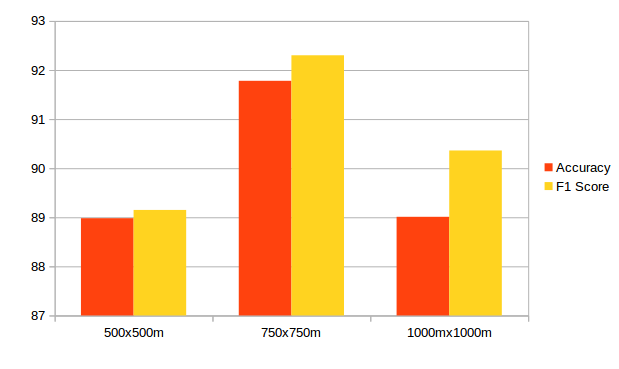
\includegraphics[width=12cm]{dimensions-experiments}
    \caption{Comparison of the Accuracy and F1 Score of the model for different cell dimensions.}
    \end{figure}
    The graph shown in Figure 4.1 compares the accuracy and F1 score of the model for the different cell dimensions. As can be seen, the model in 750mx750m cell dimension performs better in both metrics. The model in 500mx500m cell dimension has almost the same accuracy with the model in 1000mx1000m, with the latter having a higher F1 score.

    \begin{figure}[H]
    \centering
    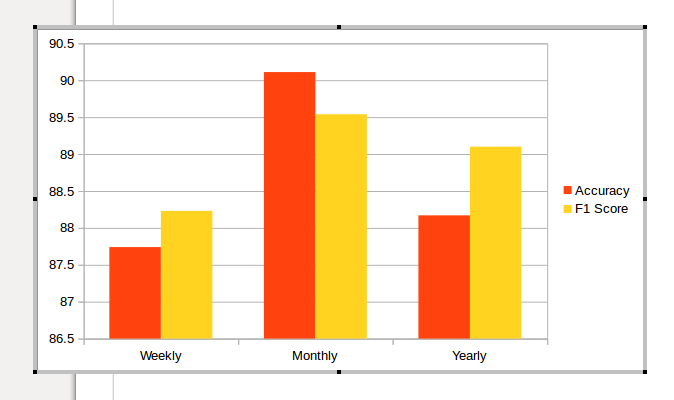
\includegraphics[width=12cm]{timestep-experiment}
    \caption{Comparison of the Accuracy and F1 Score of the model for timesteps.}
    \end{figure}
    Figure 4.2 above compares the accuracy and F1 score of the model for the different timesteps. The model in monthly timestep performs better in both accuracy and F1 score while the model in weekly timestep performs the worst.
    
    \begin{figure}[H]
    \centering
    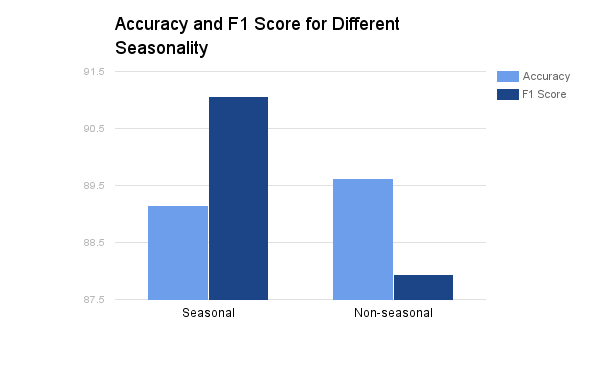
\includegraphics[width=12cm]{seasonal-experiments}
    \caption{Comparison of the Accuracy and F1 Score of the model for seasonal and non-seasonal data.}
    \end{figure}
    Figure 4.3 above compares the accuracy and F1 score of the model for seasonal and non-seasonal data. The model using seasonal data performs a little better in terms of F1 score compared to the model using non-seasonal data. The accuracy of both models have little difference.

\section{Error Analysis}
